\documentclass[12pt,journal,nofonttune]{IEEEtran}

\usepackage{booktabs} % For formal tables
\usepackage{hyperref}
\usepackage{graphicx}
\usepackage{amsmath, bm}
\usepackage{float}
\usepackage{upgreek}
\usepackage{amssymb}


\begin{document}




\section{Data Preprocessing}

Pandas will load the dataset. It could find there are $367230\times12$ data in this dataset after statistics. Also, there is missing value in ContractType, ContractTime and Company which shows in Table\ref{train_data} and Table\ref{test_data}.

\begin{table}[htbp]
\centering
\caption{The statistics of the original trainning dataset}
\label{train_data}
\begin{tabular}{|c|c|c|}
 \hline
   & Id                 & 244767 non-null int64  \\
 \hline
   & Title              & 244767 non-null object \\
 \hline
   & FullDescription    & 244767 non-null object \\
 \hline
   & LocationRaw        & 244767 non-null object \\
 \hline
   & LocationNormalized & 244767 non-null object \\
 \hline
 Training data & ContractType       & 65442 non-null object \\
 \hline
   & ContractTime       & 180863 non-null object \\
 \hline
   & Company            & 212338 non-null object \\
 \hline
   & Category           & 244767 non-null object \\
 \hline
   & SalaryRaw          & 244767 non-null object \\
 \hline
   & SalaryNormalized   & 244767 non-null object \\
 \hline
   & SourceName         & 244767 non-null object \\
 \hline
\end{tabular}
\end{table}

\begin{table}[htbp]
\centering
\caption{The statistics of the original testing dataset}
\label{test_data}
\begin{tabular}{|c|c|c|}
 \hline
   & Id                   & 122463 non-null int64  \\
 \hline
   & Title                & 122463 non-null object \\
 \hline
   & FullDescription      & 122463 non-null object \\
 \hline
   & LocationRaw          & 122463 non-null object \\
 \hline
   & LocationNormalized   & 122463 non-null object \\
 \hline
 Testing data & ContractType    & 33013 non-null object  \\
 \hline
   & ContractTime         & 90702 non-null object  \\
 \hline
   & Company              & 106202 non-null object \\
 \hline
   & Category             & 122463 non-null object \\
 \hline
   & SalaryRaw            & NA                     \\
 \hline
   & SalaryNormalized     & NA                     \\
 \hline
   & SourceName           & 122463 non-null object \\
 \hline
\end{tabular}
\end{table}

\begin{itemize}
\item Clustering

\ \ Openrefine is a data transforming tool which could search, clean and integrate data\cite{verborgh2013using}. In this project, the missing value will be filled by this tool and the string data will be clustered which is shown in Fig\ref{cluster}.

\begin{figure}[htbp]
    \centering
    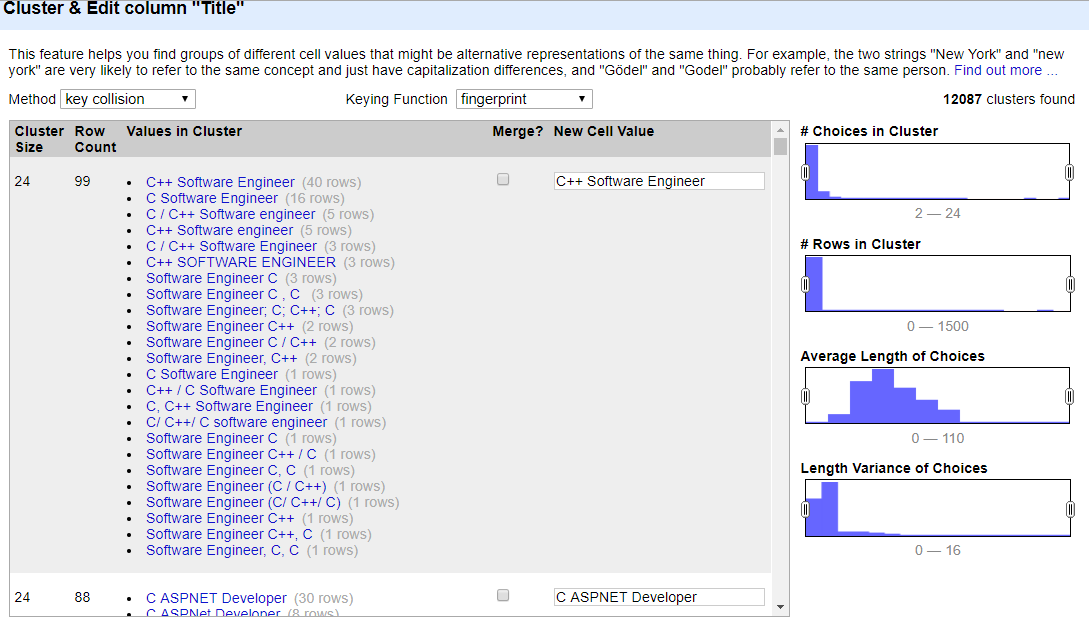
\includegraphics[width=0.55\textwidth]{cleaning_step1.png}
    \caption{\label{cluster}Clustering function in Openrefine}
\end{figure}

\item Location match

\ \ Location tree is a supplemental dataset which contains the hierarchical relationship between the different Normalized Locations of the original dataset. Therefore, the longest word in each data of LocaitonNormalized will be used to match the information in location tree.

\item Coding and One-hot-vector

\ \ For the information in FullDescription, the HasingVectrizer of sklearn will be used to process string information with Hash coding.
Each cluster of attributes will be coded with a unique digital. Due to there are too many clusters in Title, Location and Company, only the number of cluster bigger than ten will be counted as valid clusters. 
After coding, the one-hot encoding module in Keras will be used to generate the one-hot vector of unique digital.
\end{itemize}

After data preprocessing, the orgiAfter data preprocessing, the original dataset is transforming to digital dataset with shape of $367230\times9736$.

\section{KNN(k-nearest neighbors algorithm)}

When training dataset with given tags, the feature of test data can be compared with features in training data. Then, the top K of most similar features in training dataset will be calculated and the test data will be classified to the most frequently occurring tags\cite{zhang2007ml}.
The algorithm is described as:

\begin{itemize}
\item[1] Calculate the distance between test data and each training data.
\item[2] Sort by the relationship of increasing distance.
\item[3] Select the K points which have the smallest distance.
\item[4] Determine the occurred frequency of the top K points.
\item[5] Returns the most frequent category of the top K points as a predictive classification.
\end{itemize}
\ \ The training data will be divided into ten groups by KFold and the Grid Search in sklearn will be used to find the best value of K in KNN. In this project, the best parameter of K is 1. Therefore, training all data with one neighbor and the mean difference of predicting salary is 15850.69. This result is unsatisfactory because the dimensional of data is high and KNN will give an existing salary(tag) in training data which will also cause the error.

\section{NN(Artificial neural network)}

Several models were built by Keras in this part. Due to the page limitation, the model with the best performance will be introduced. Fig\ref{model} shows the configuration of this model. 

\begin{itemize}
\item It uses Sequential model for building and the dense is full connected layers which could represent different weights. 
\item Batch normalization is using to adjust the parameters between layers by zero mean value and one variance\cite{ioffe2015batch}. In this project, the convergence speed increased striking with BN preprocessing.
\item Rectified Linear Unit(ReLU) is used as activating the function to add a non-linear parameter to dense. It has six times convergence speed compared to sigmoid and tanh function and it could reduce the vanishing gradient\cite{ruder2016overview}.
\item Dropout means the connection between each neural has a disconnected probability which could reduce the complexity of the model to prevent overfitting\cite{srivastava2014dropout}. Also, and the call back function is used to avoid overfitting with early stopping as well.
\end{itemize}

\begin{figure}[htbp]
    \centering
    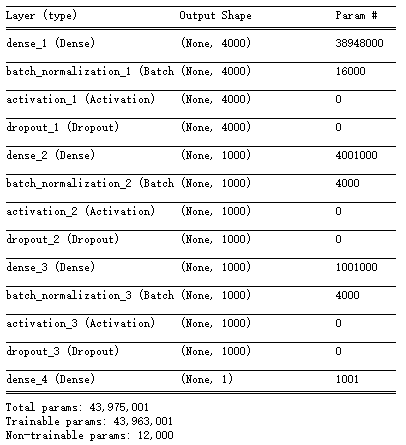
\includegraphics[width=0.4\textwidth]{model.png}
    \caption{\label{model}Structure of training model}
\end{figure}

Three optimizers were tested in this project which are sgd(mini-batch gradient descent), Adadelta and Adam(Adaptive Moment Estimation). Adam had a higher convergence speed, but sgd had a higher accuracy. 

Therefore, the final configuration is a three layers model with sgd optimizer. After epochs 2000, the changing in mean squared error of model is shown in Fig\ref{loss}. It could find the convergence speed is decreased with epoch’s increasing, this is because the learning rate is a constant in this project. The MSE of this model still decreases, however, due to the time limitation and the slow convergence speed. The training stops at epochs 2000. Comparing with KNN, the predicted salary of this NN model has outstanding progress. The mean difference of this model is 9275.03 which could rank 77 of this competition. In addition, the author of this competition did not provide exact salary information of test dataset but give a predicted result with the Random solemnity which means the mean difference may reduce with real data.


\begin{figure}[htbp]
    \centering
    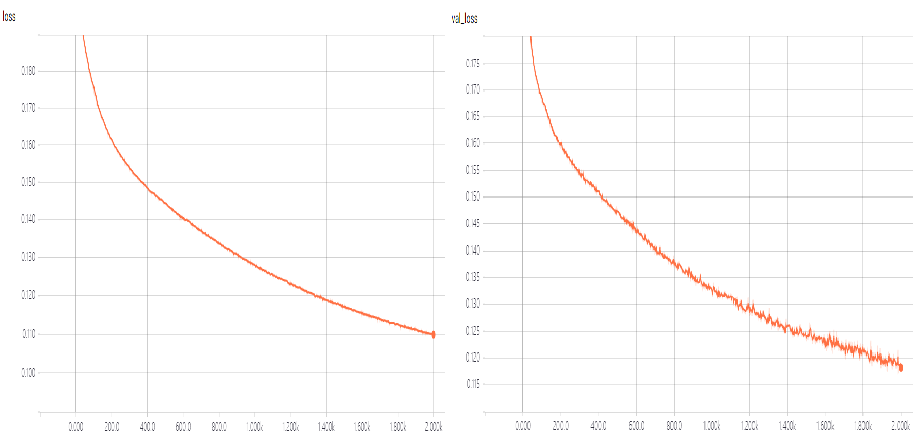
\includegraphics[width=0.55\textwidth]{loss.png}
    \caption{\label{loss}MSE changing of training data and valid data in epoch 2000}
\end{figure}


\bibliographystyle{IEEEtran}
\bibliography{MLZJM}

\end{document}